\chapter{\IfLanguageName{dutch}{Figuren: Vergelijkende Studie}{Comparitive Study Figures}}%
\label{ch:afbeeldingen-resultaten-verg-studie}


\begin{table}[h]
	\centering
	\begin{tabular}{ | m{3cm} | m{3cm} | m{3cm} | } 
		\hline
		Bron & #Zinnen in A1 & #Zinnen in A2 \\
		\hline
		Oorspronkelijk & 78  & 159 \\ 
		\hline
		MTS (door leerkracht) & 43 & 45 \\
		\hline
		MTS (door leerling) & n.v.t. & 50 \\
		\hline
		T1 & 101 & 209 \\
		\hline
		T2 & 82 & 209 \\
		\hline
		T3 & 100 & 209 \\
		\hline
		T4 P1 & 61 & 98 \\
		\hline
		T4 P2 & 89 & 133 \\
		\hline
		T4 P3 & 39 & 55 \\
		\hline
	\end{tabular}
	\label{table:resultaten-aantal-zinnen}
	\caption{Aantal zinnen (gemeten met Spacy sentence embeddings) per tekst.}
\end{table}


\begin{figure}
	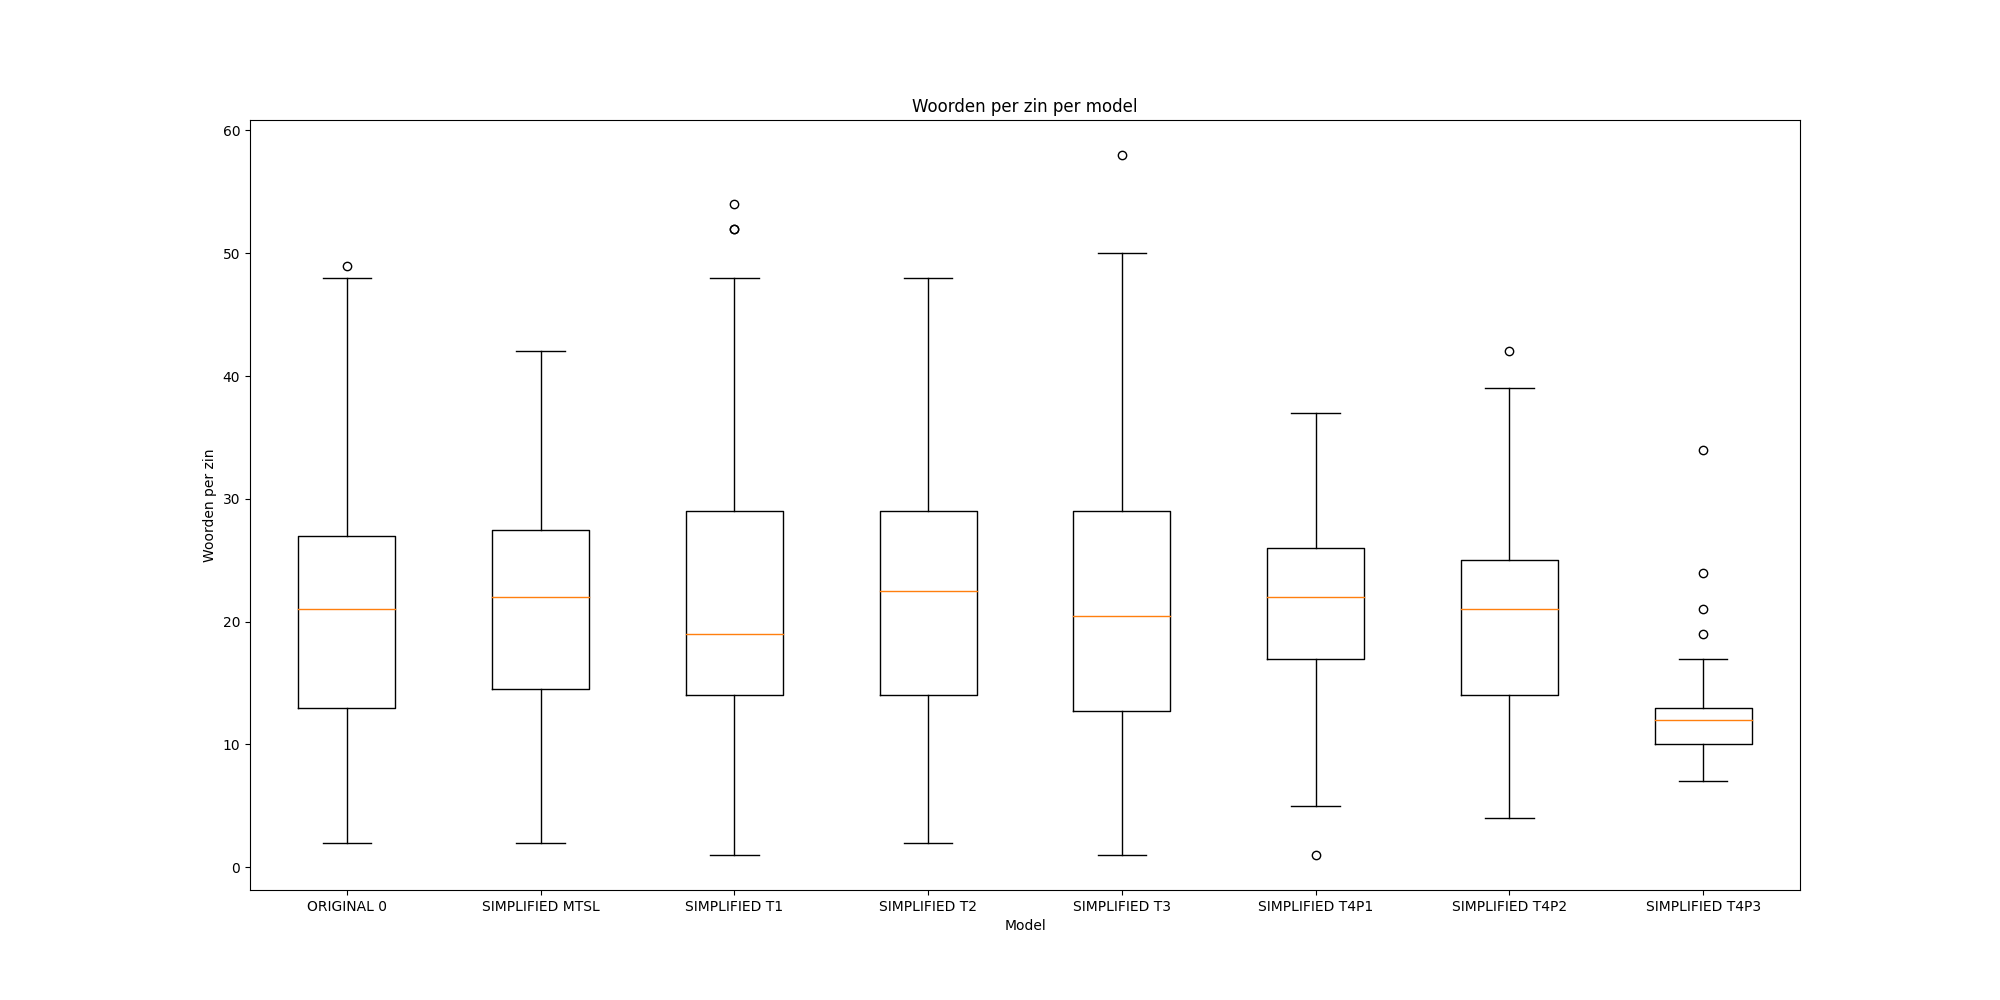
\includegraphics[width=\linewidth]{img/boxplot-avg-a1.png}
	\caption{Overzicht van het minimum, maximum en gemiddeld aantal woorden per zin per model in A1.}
	\label{img:boxplot-min-max-avg-words-a1}
\end{figure}

\begin{figure}
	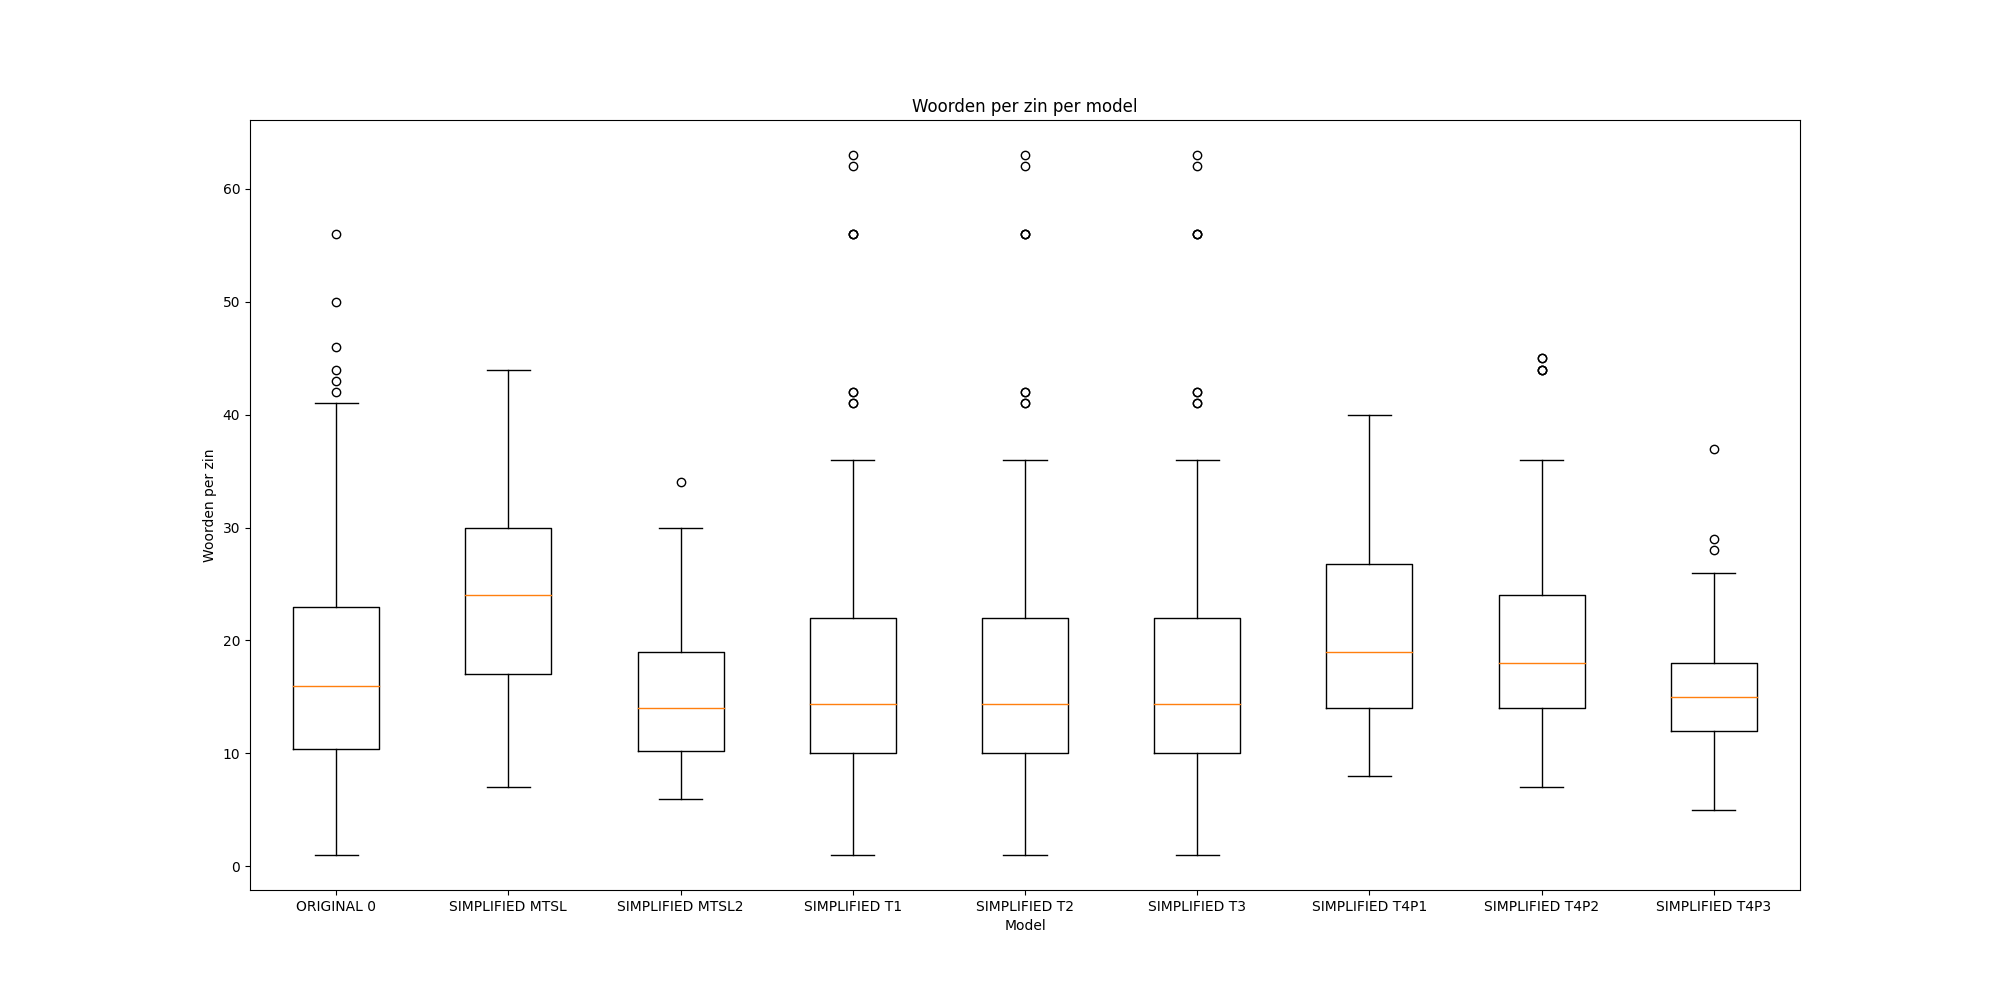
\includegraphics[width=\linewidth]{img/boxplot-avg-a2.png}
	\caption{Overzicht van het minimum, maximum en gemiddeld aantal woorden per zin per model in A2.}
	\label{img:boxplot-min-max-avg-words-a2}
\end{figure}


\begin{figure}
	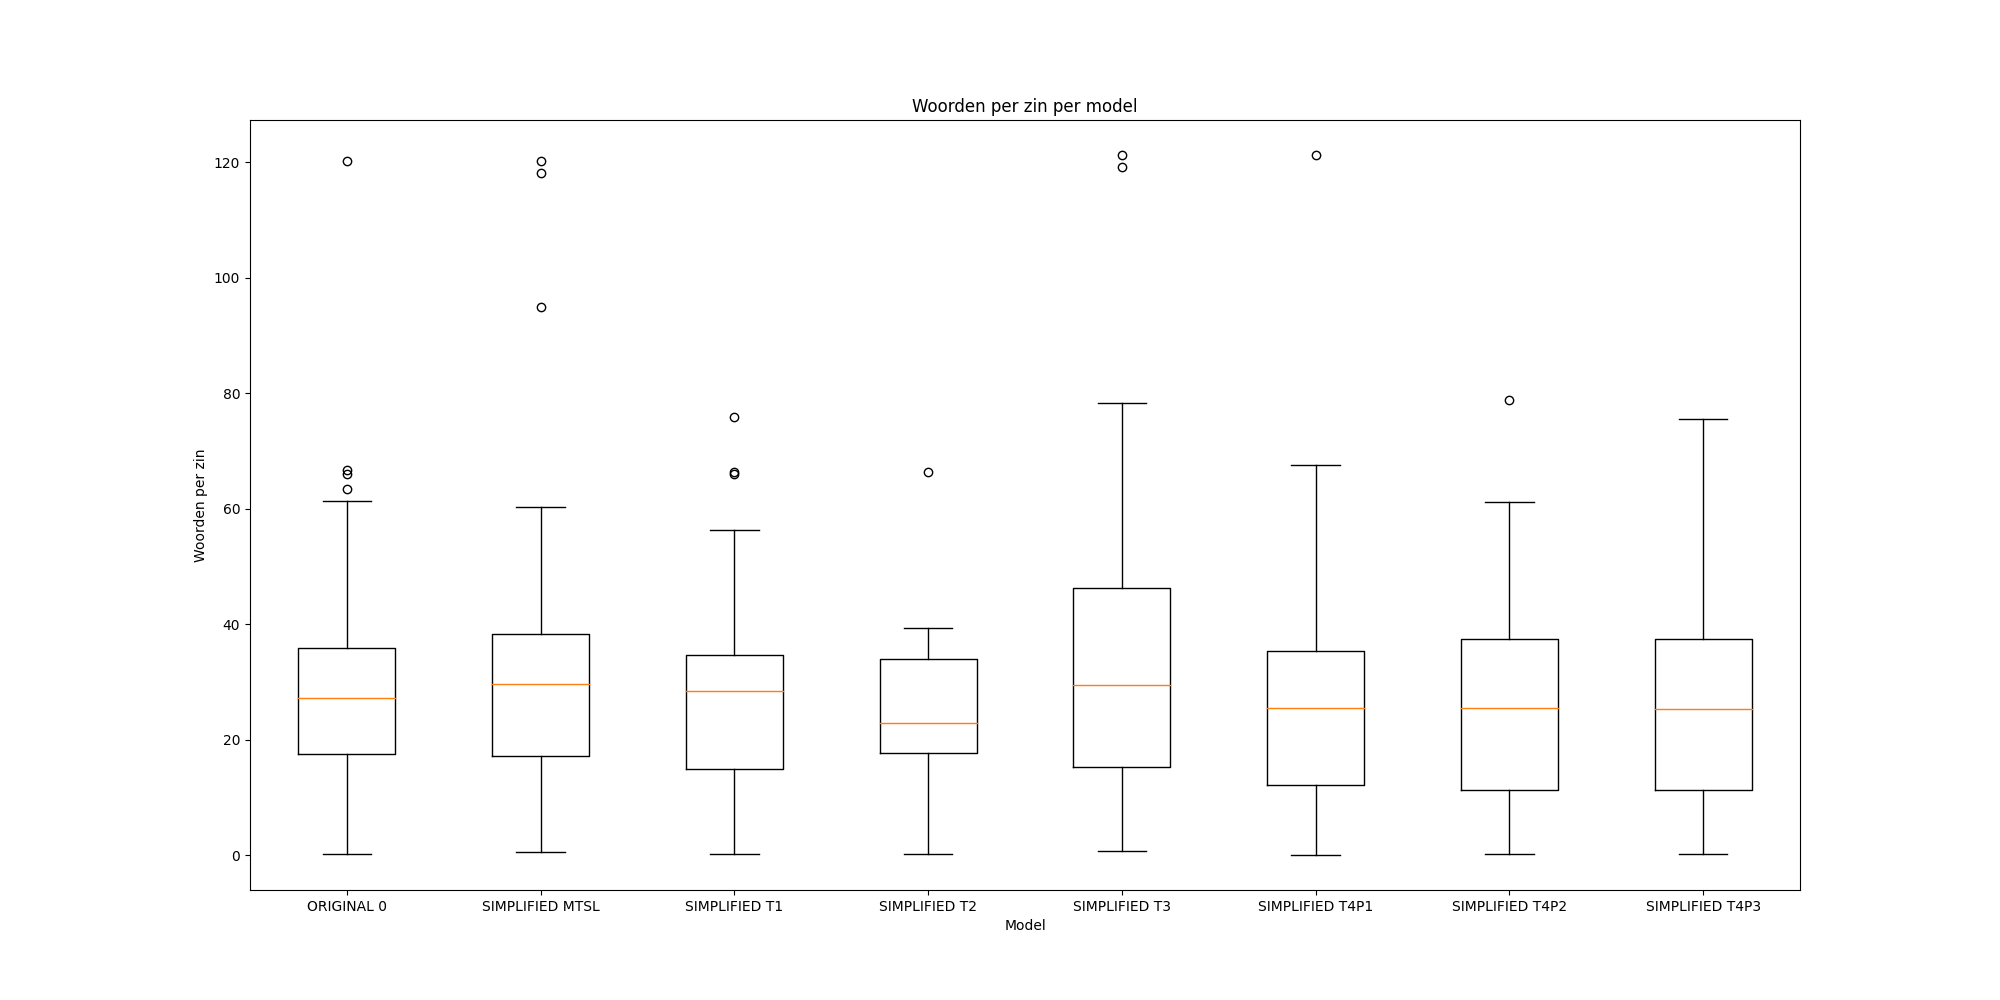
\includegraphics[width=\linewidth]{img/boxplot-fre-a1.png}
	\caption{Boxplot van de FRE-scores voor A1.}
	\label{img:boxplot-fre-a1}
\end{figure}

\begin{figure}
	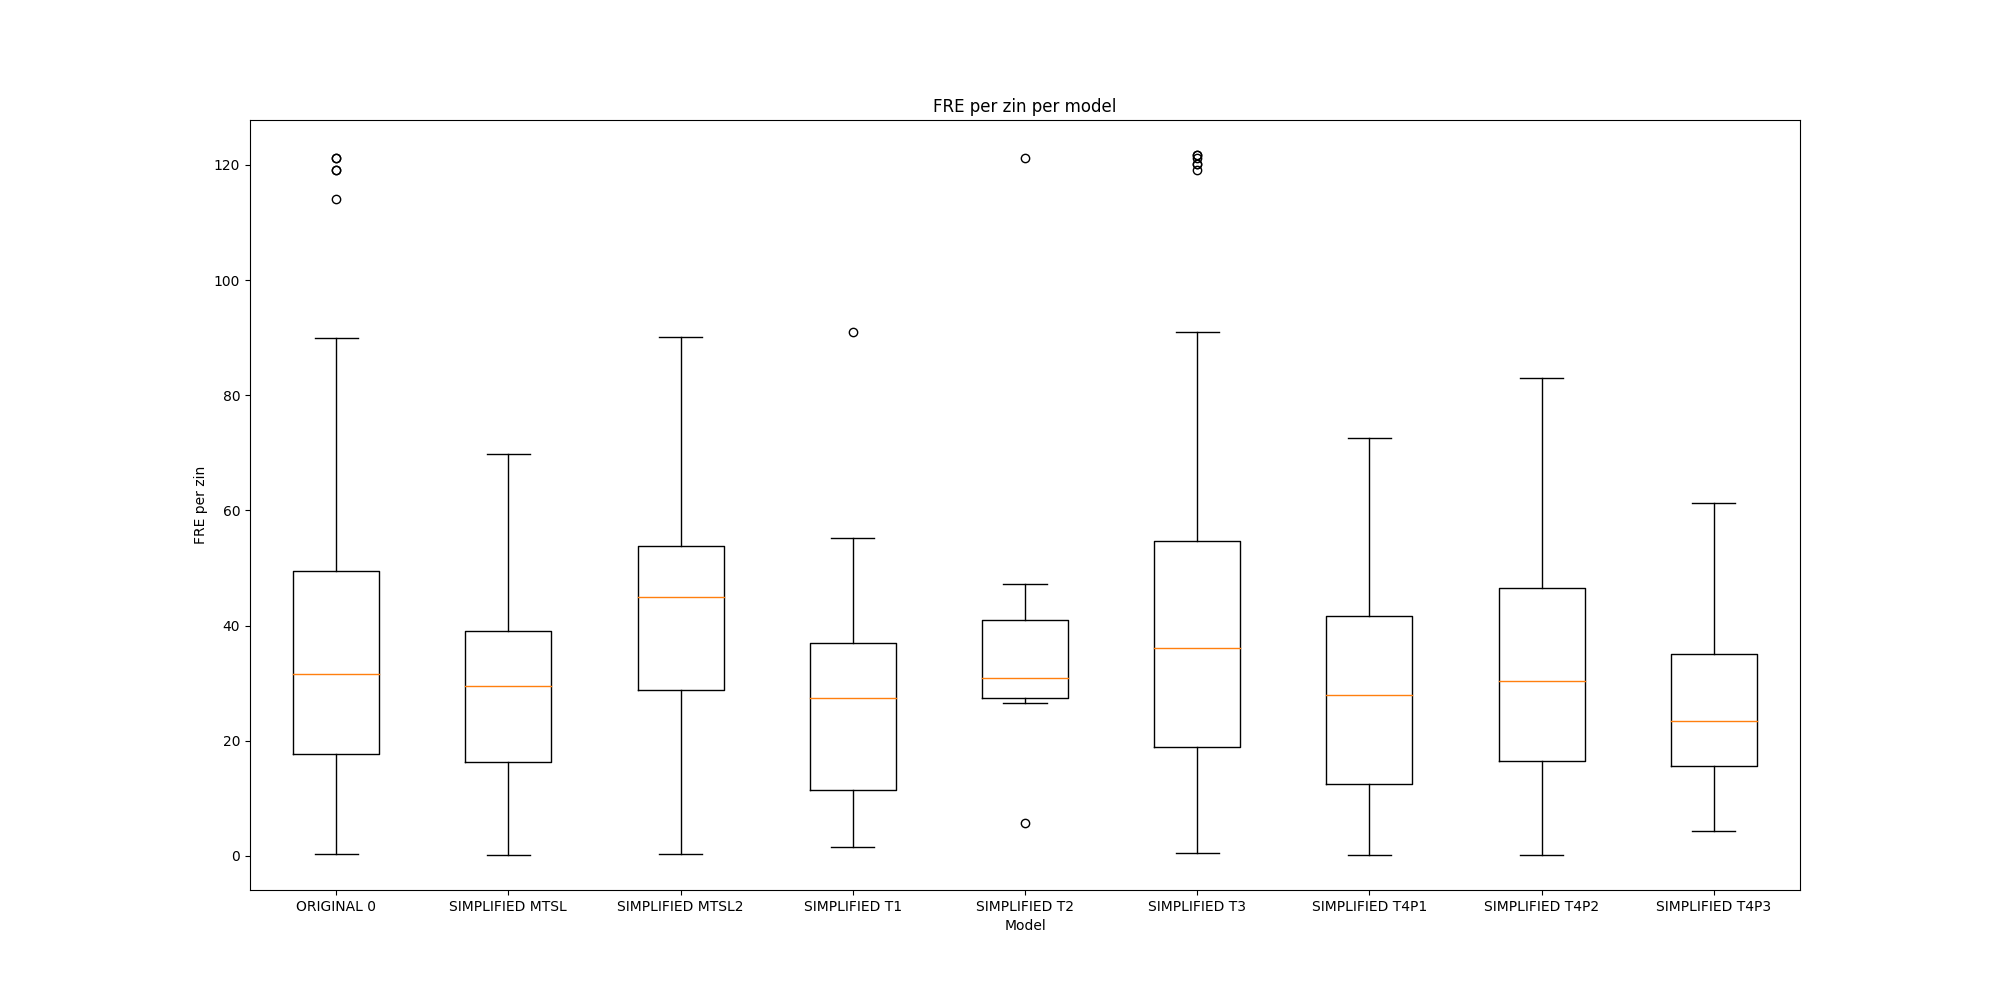
\includegraphics[width=\linewidth]{img/boxplot-fre-a2.png}
	\caption{Boxplot van de FRE-scores voor A2.}
	\label{img:boxplot-fre-a2}
\end{figure}

\begin{figure}
	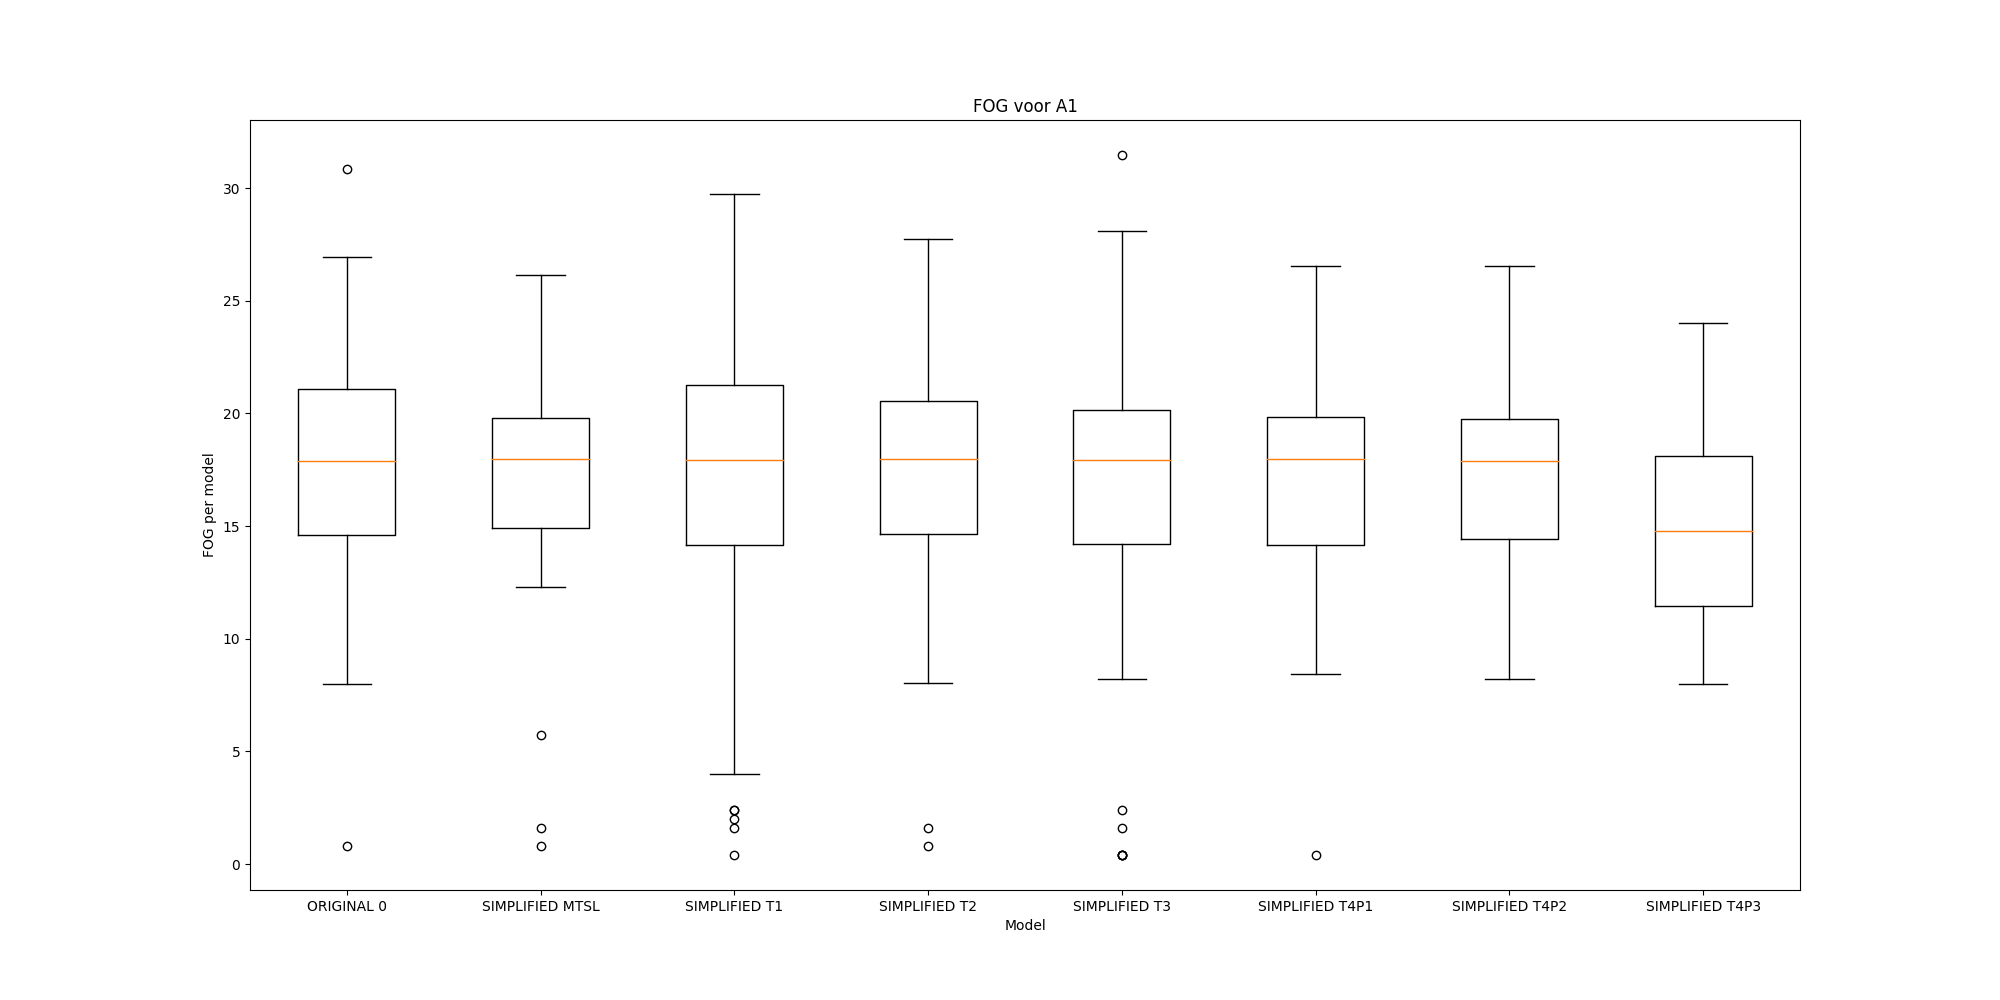
\includegraphics[width=\linewidth]{img/boxplot-fog-a1.png}
	\caption{Boxplot van de FOG-scores voor A1.}
	\label{img:boxplot-fog-a1}
\end{figure}

\begin{figure}
	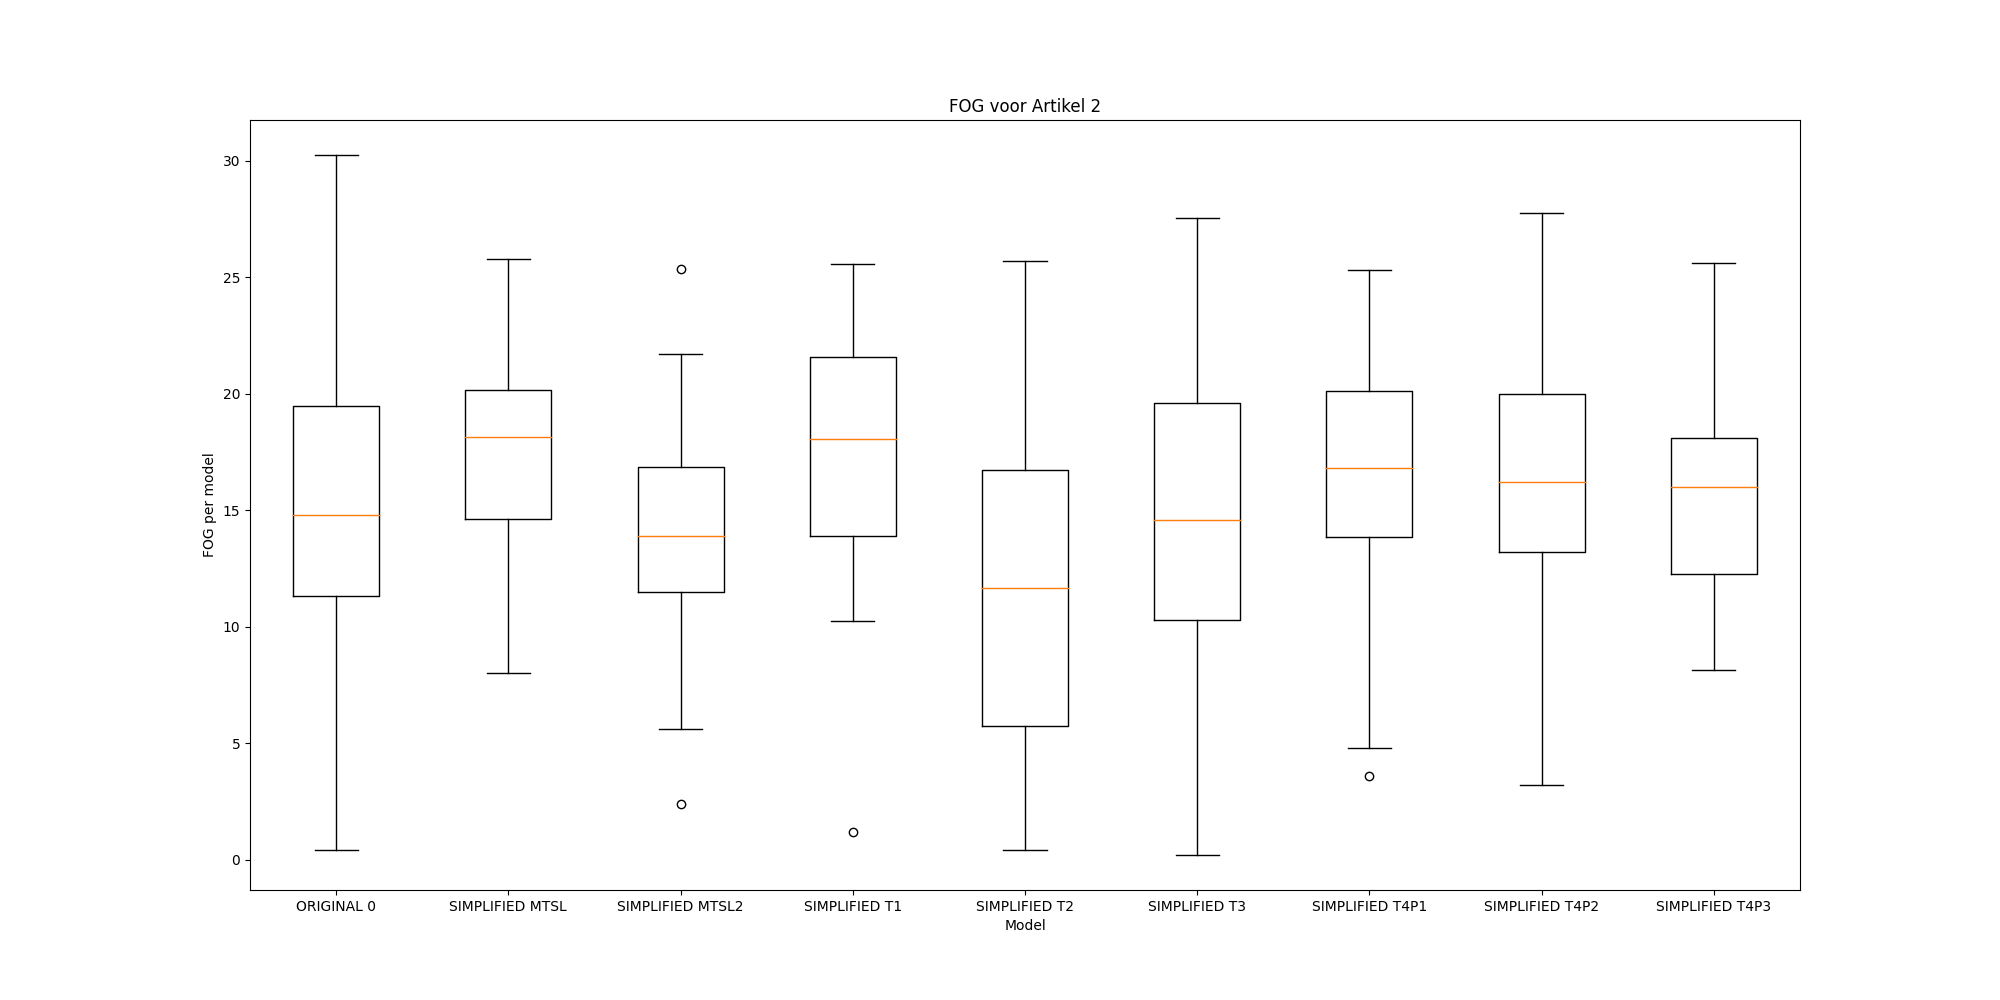
\includegraphics[width=\linewidth]{img/boxplot-fog-a2.png}
	\caption{Boxplot van de FOG-scores voor A2.}
	\label{img:boxplot-fog-a2}
\end{figure}

\begin{figure}
	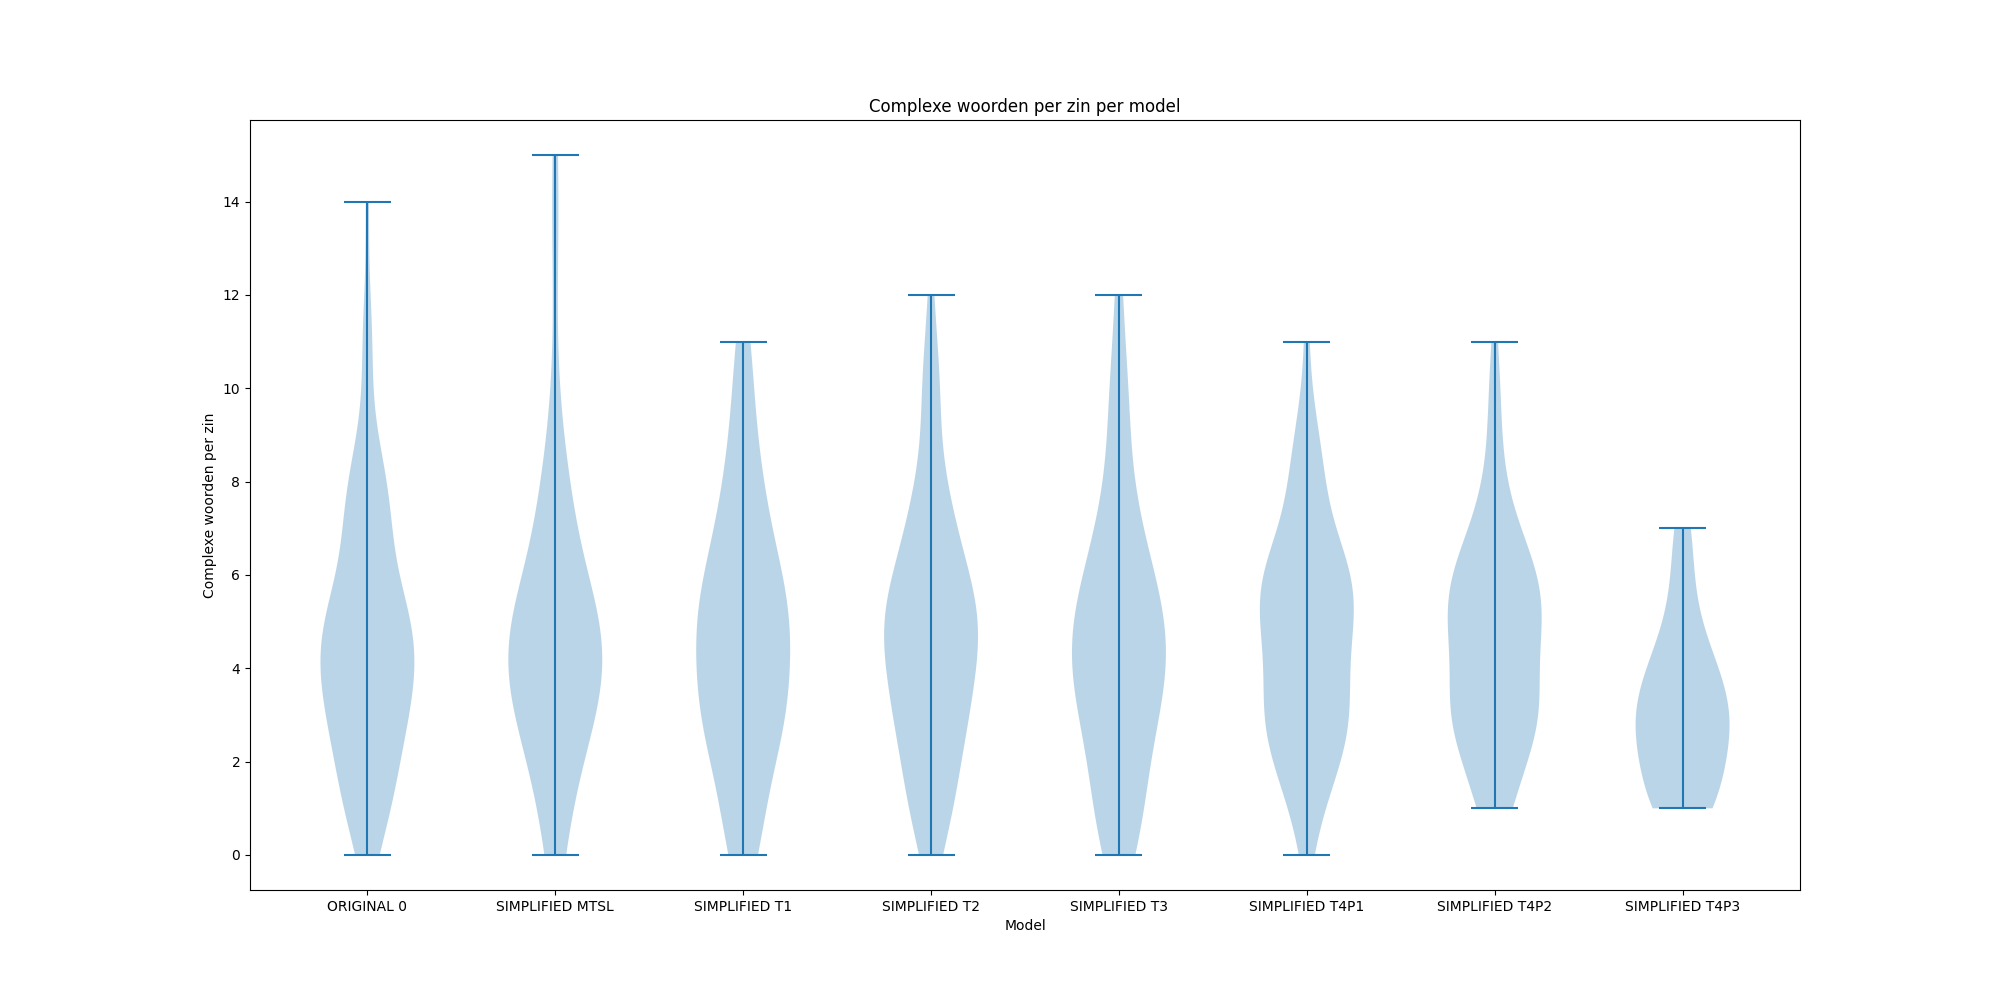
\includegraphics[width=\linewidth]{img/violinplot-complex-a1.png}
	\caption{Gemiddeld aantal complexe woorden per zin gegroepeerd op model voor A1.}
	\label{img:violinplot-complex-a1}
\end{figure}

\begin{figure}
	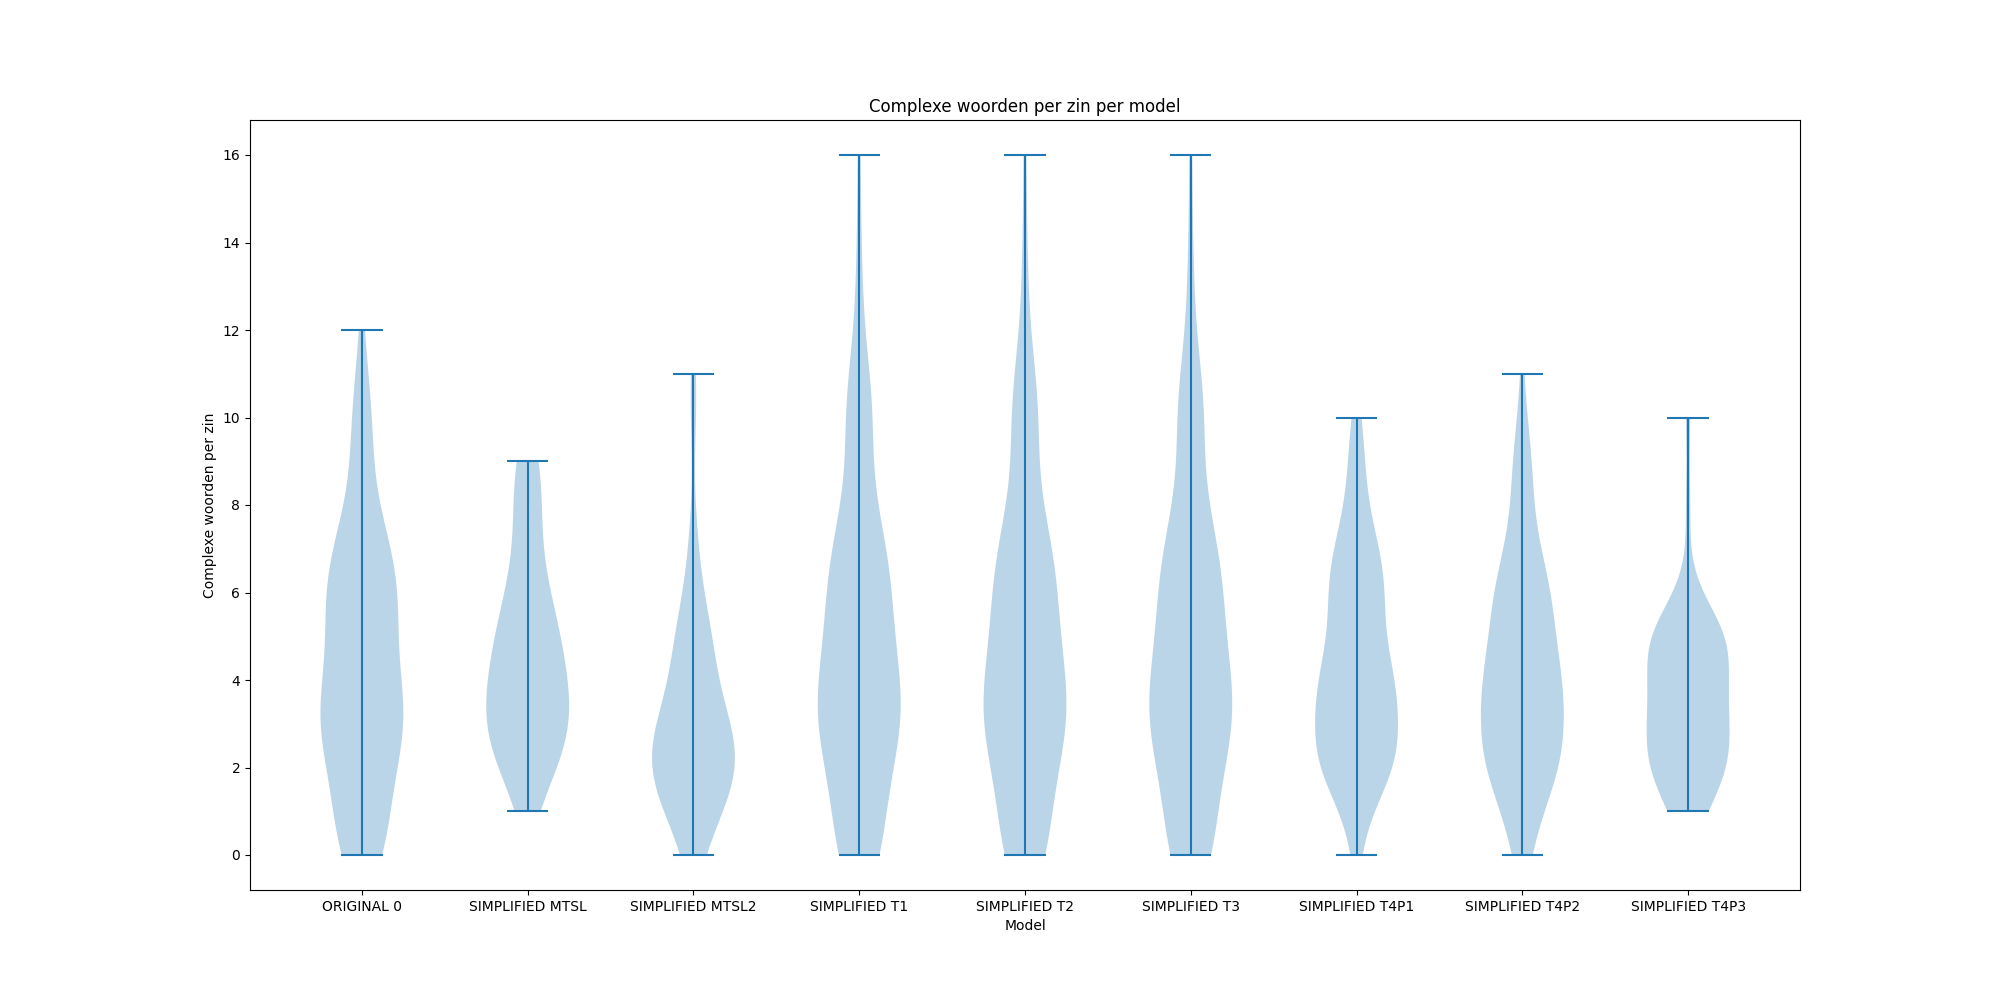
\includegraphics[width=\linewidth]{img/violinplot-complex-a2.png}
	\caption{Gemiddeld aantal complexe woorden per zin gegroepeerd op model voor A2.}
	\label{img:violinplot-complex-a2}
\end{figure}

\begin{figure}
	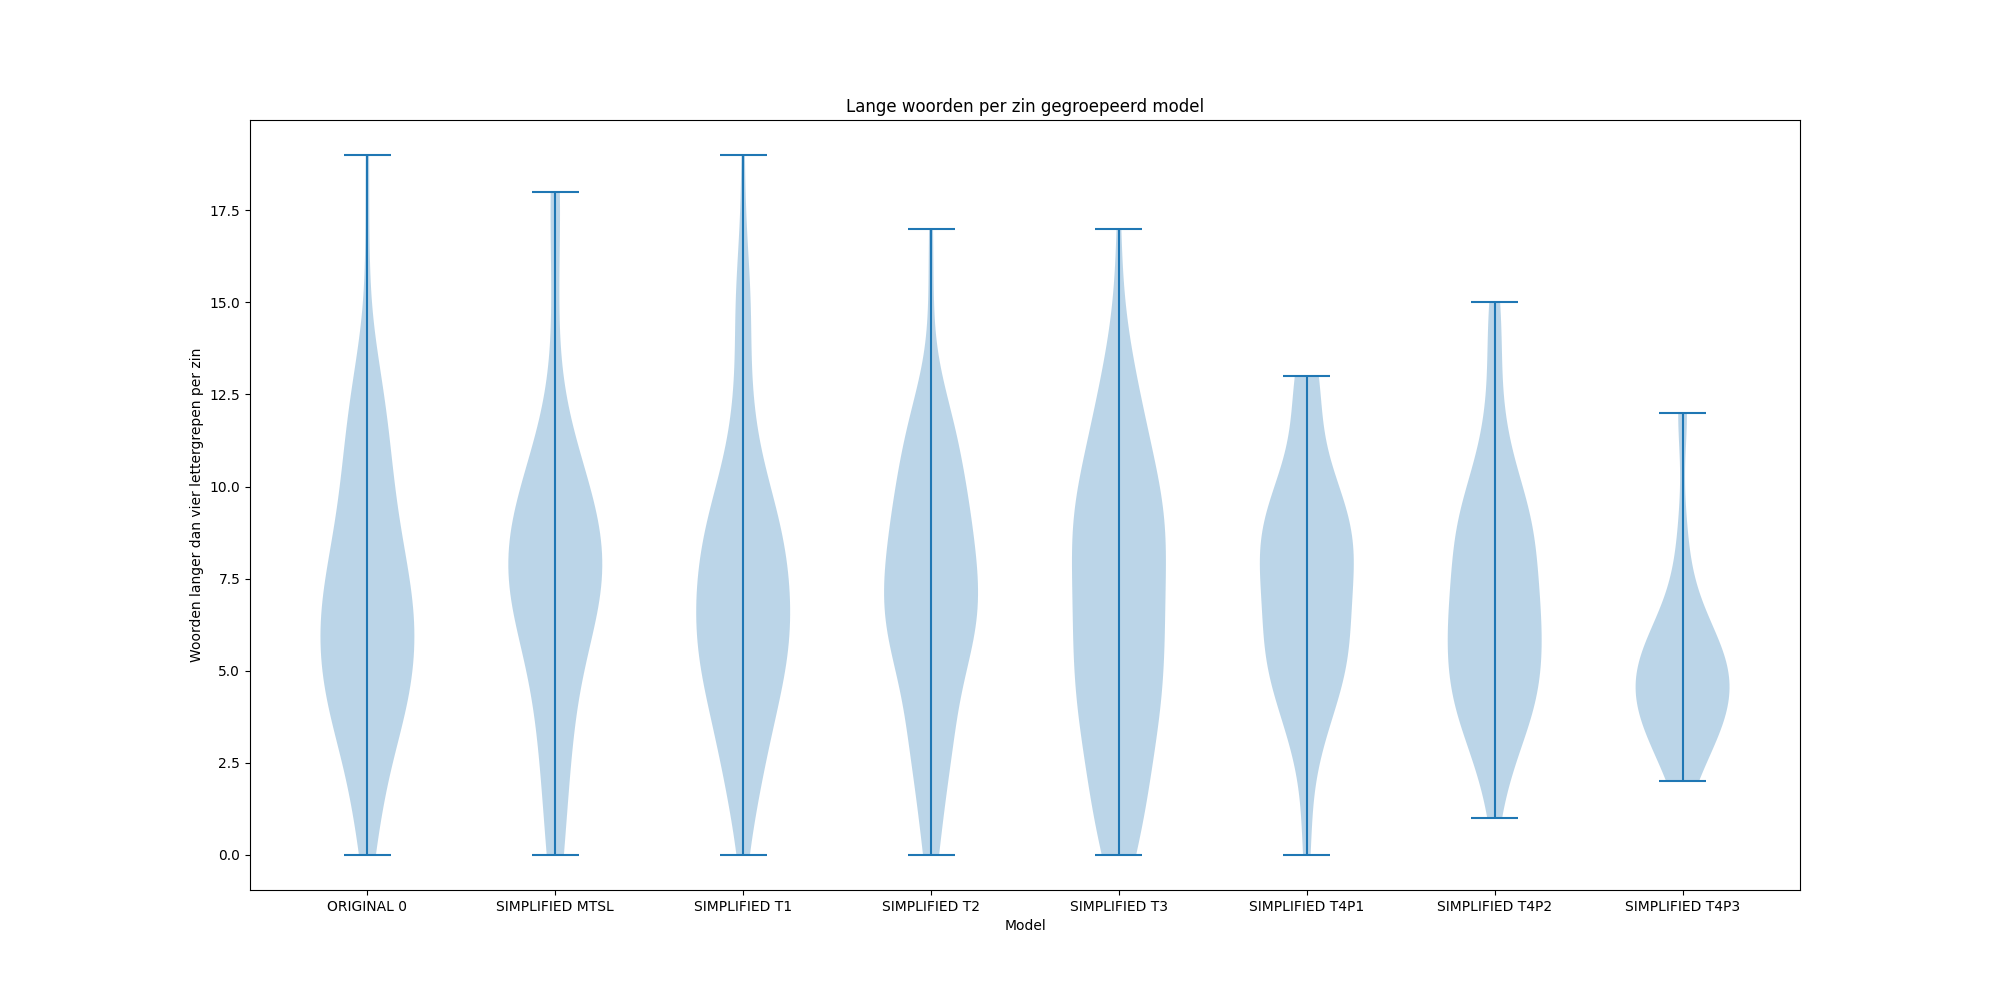
\includegraphics[width=\linewidth]{img/violinplot-long-a1.png}
	\caption{Gemiddeld aantal lange woorden per zin gegroepeerd op model voor A1.}
	\label{img:violinplot-long-a1}
\end{figure}

\begin{figure}
	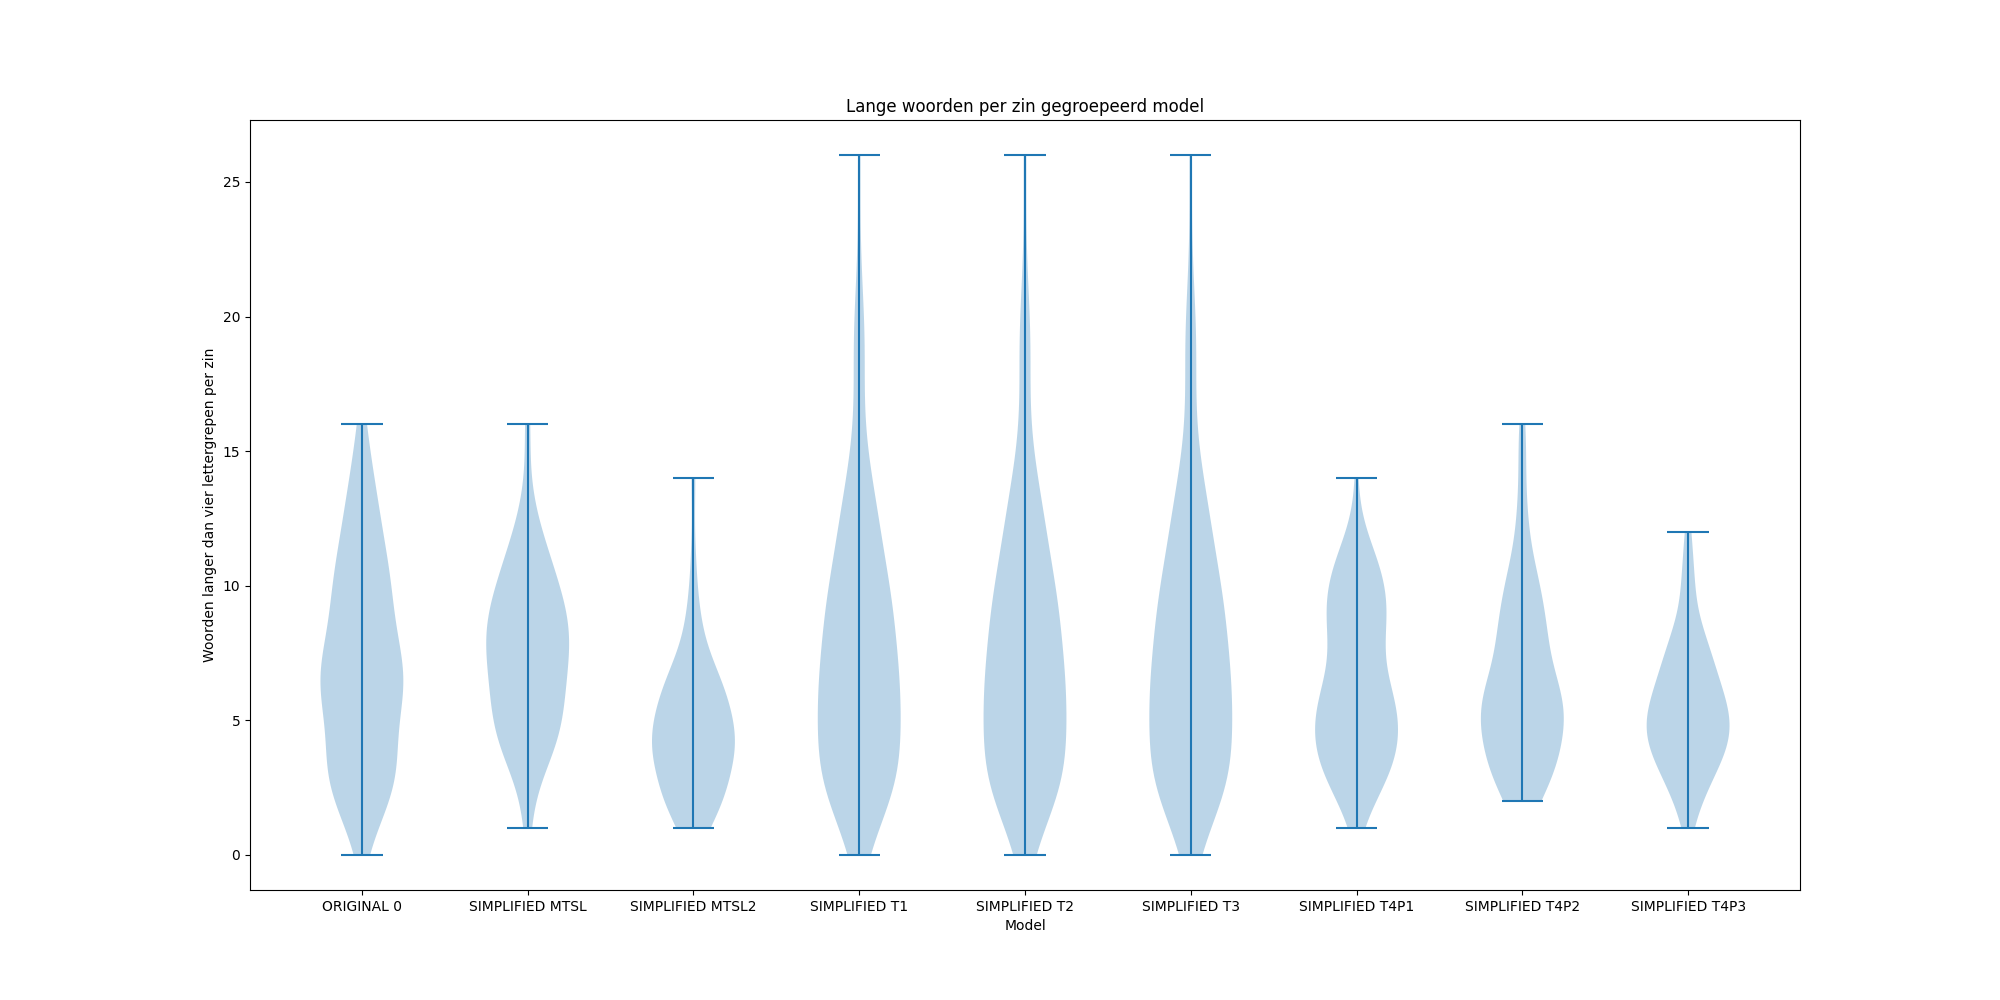
\includegraphics[width=\linewidth]{img/violinplot-long-a2.png}
	\caption{Gemiddeld aantal lange woorden per zin gegroepeerd op model voor A2.}
	\label{img:violinplot-long-a2}
\end{figure}

\begin{figure}
	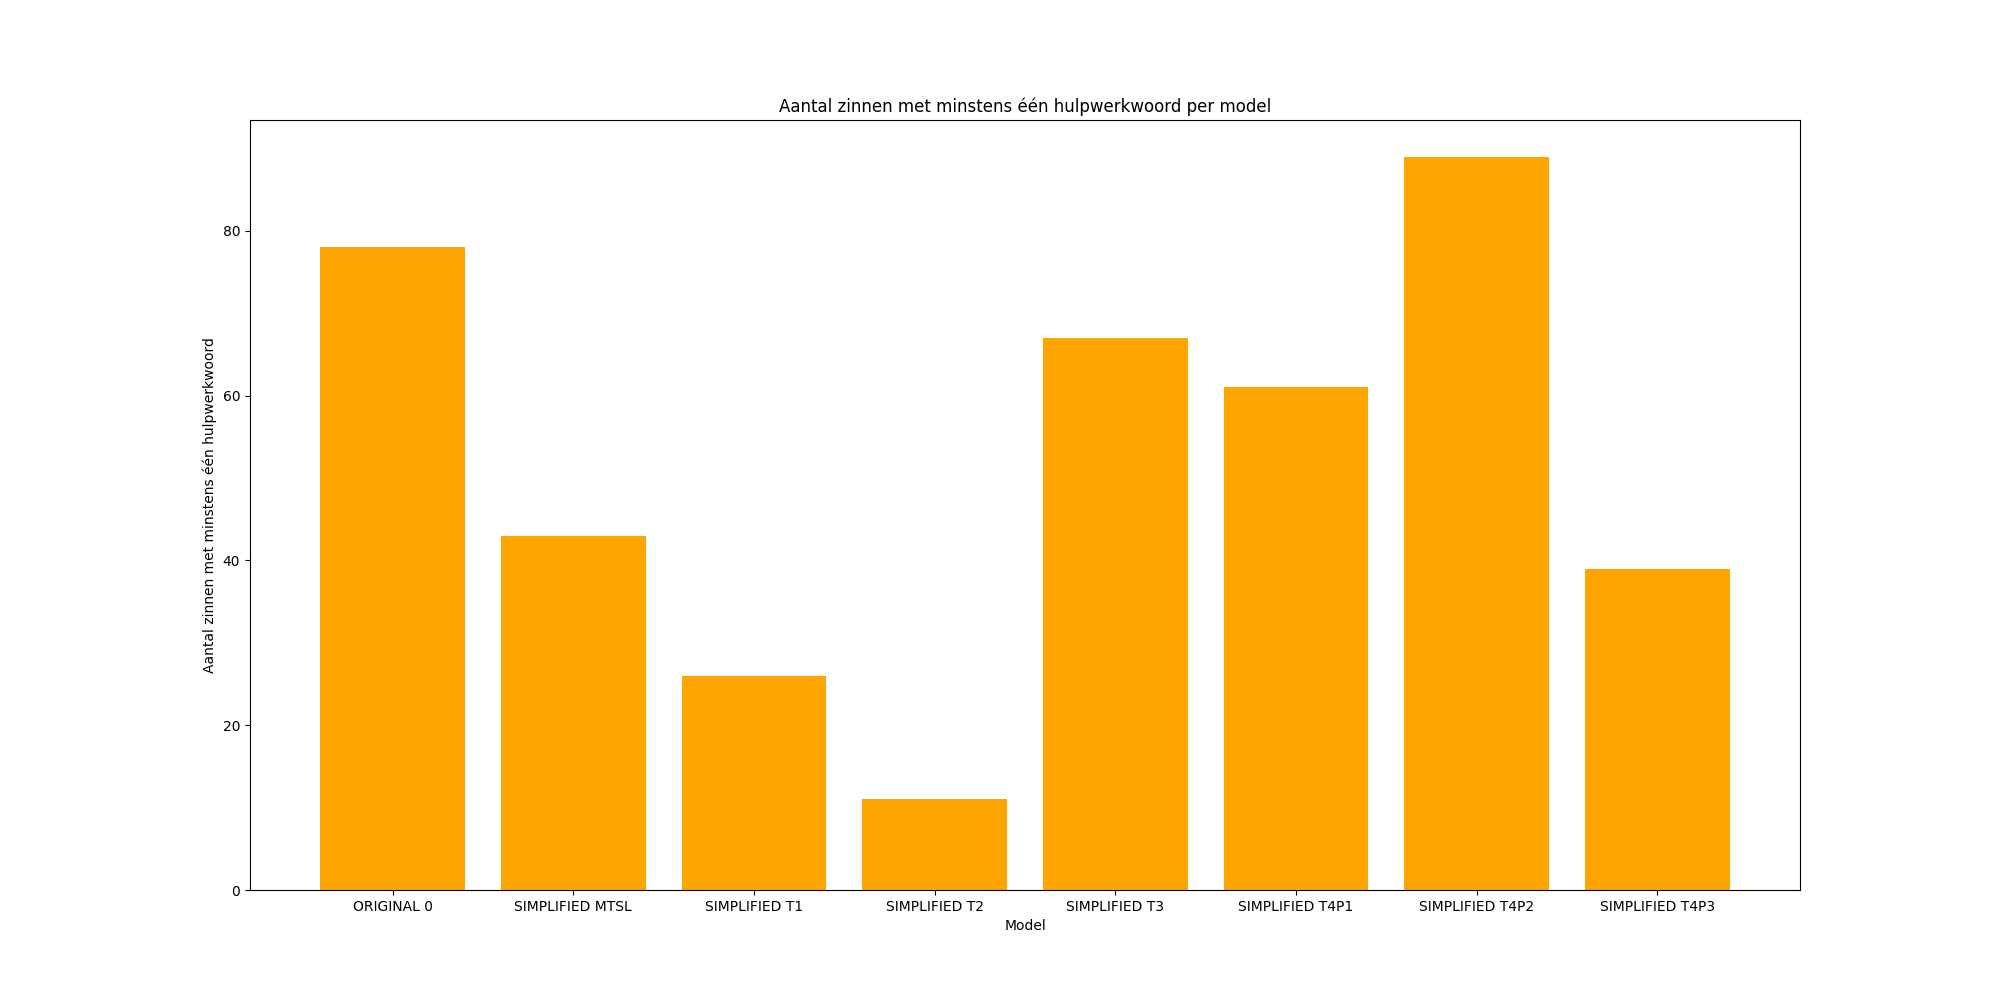
\includegraphics[width=\linewidth]{img/boxplot-aux-a1.png}
	\caption{Gemiddeld aantal hulpwerkwoorden per zin gegroepeerd op model voor A1.}
	\label{img:histplot-aux-a1}
\end{figure}

\begin{figure}
	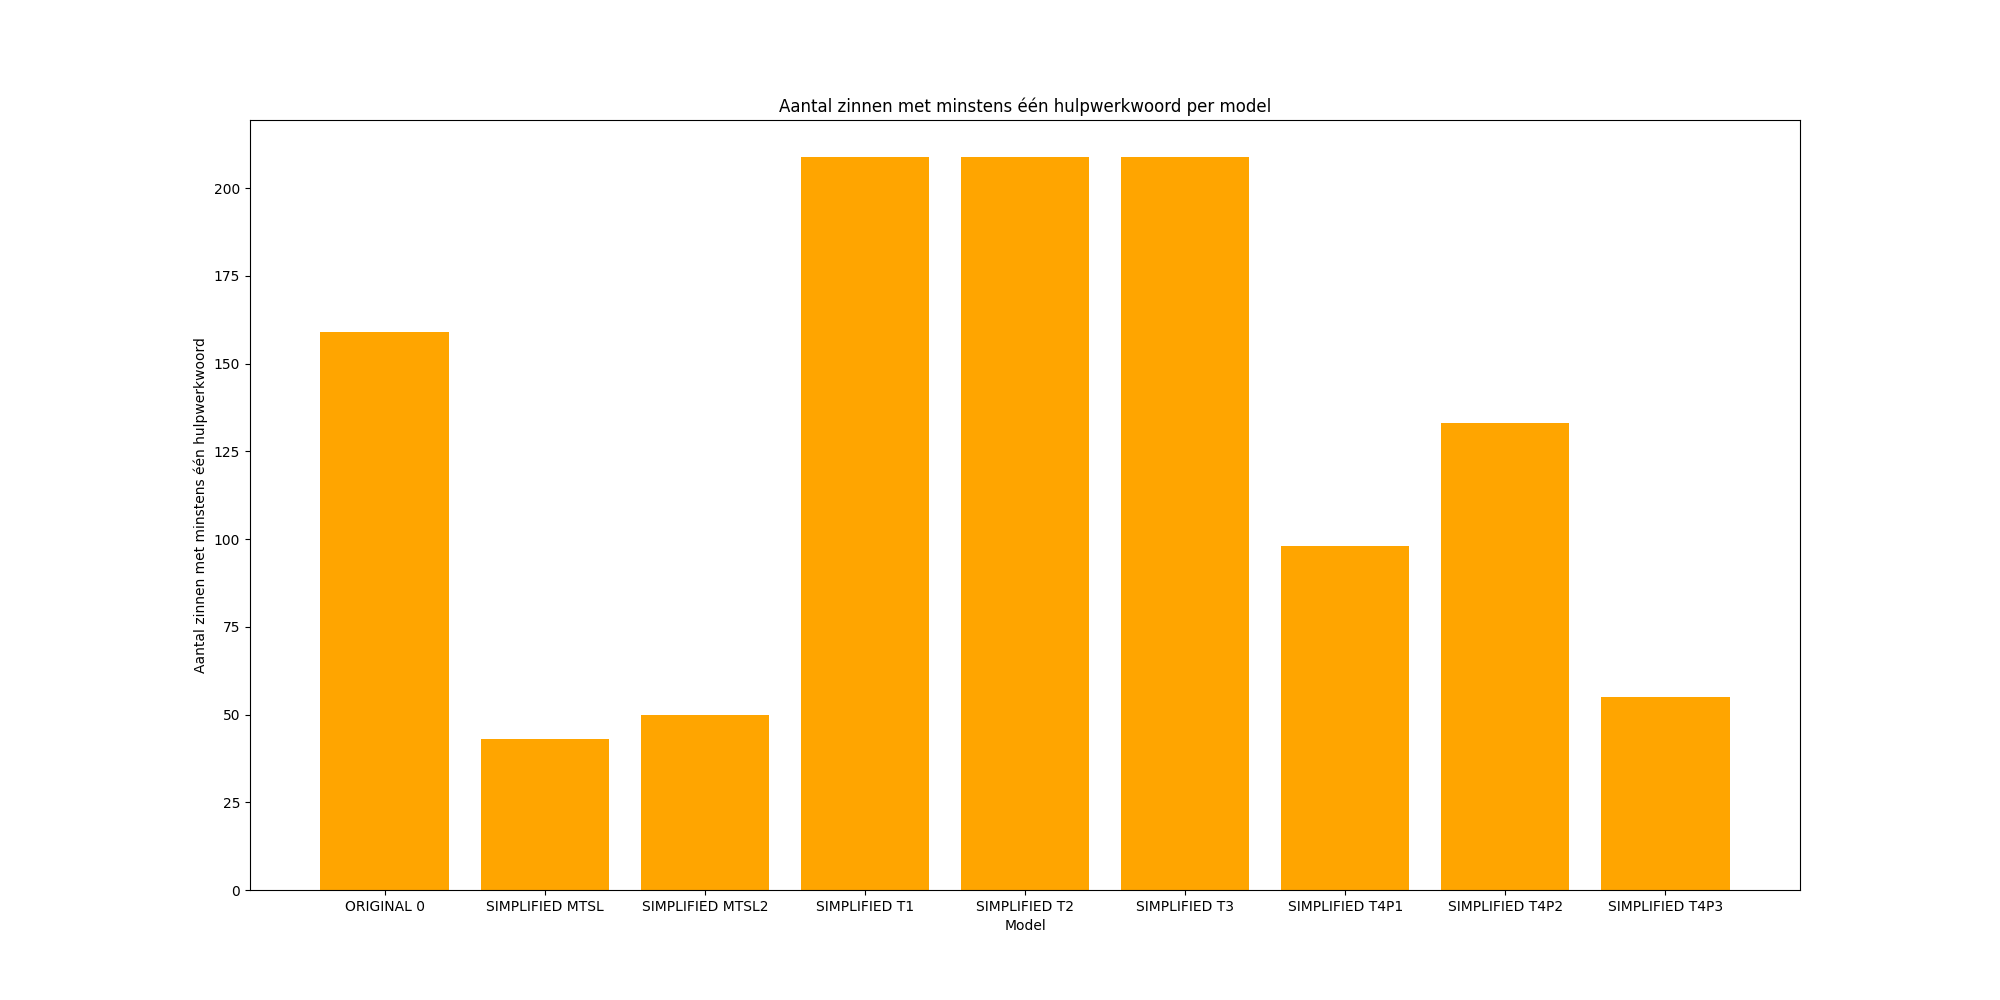
\includegraphics[width=\linewidth]{img/boxplot-aux-a2.png}
	\caption{Gemiddeld aantal hulpwerkwoorden per zin gegroepeerd op model voor A2.}
	\label{img:histplot-aux-a2}
\end{figure}

% tobe

\begin{figure}
	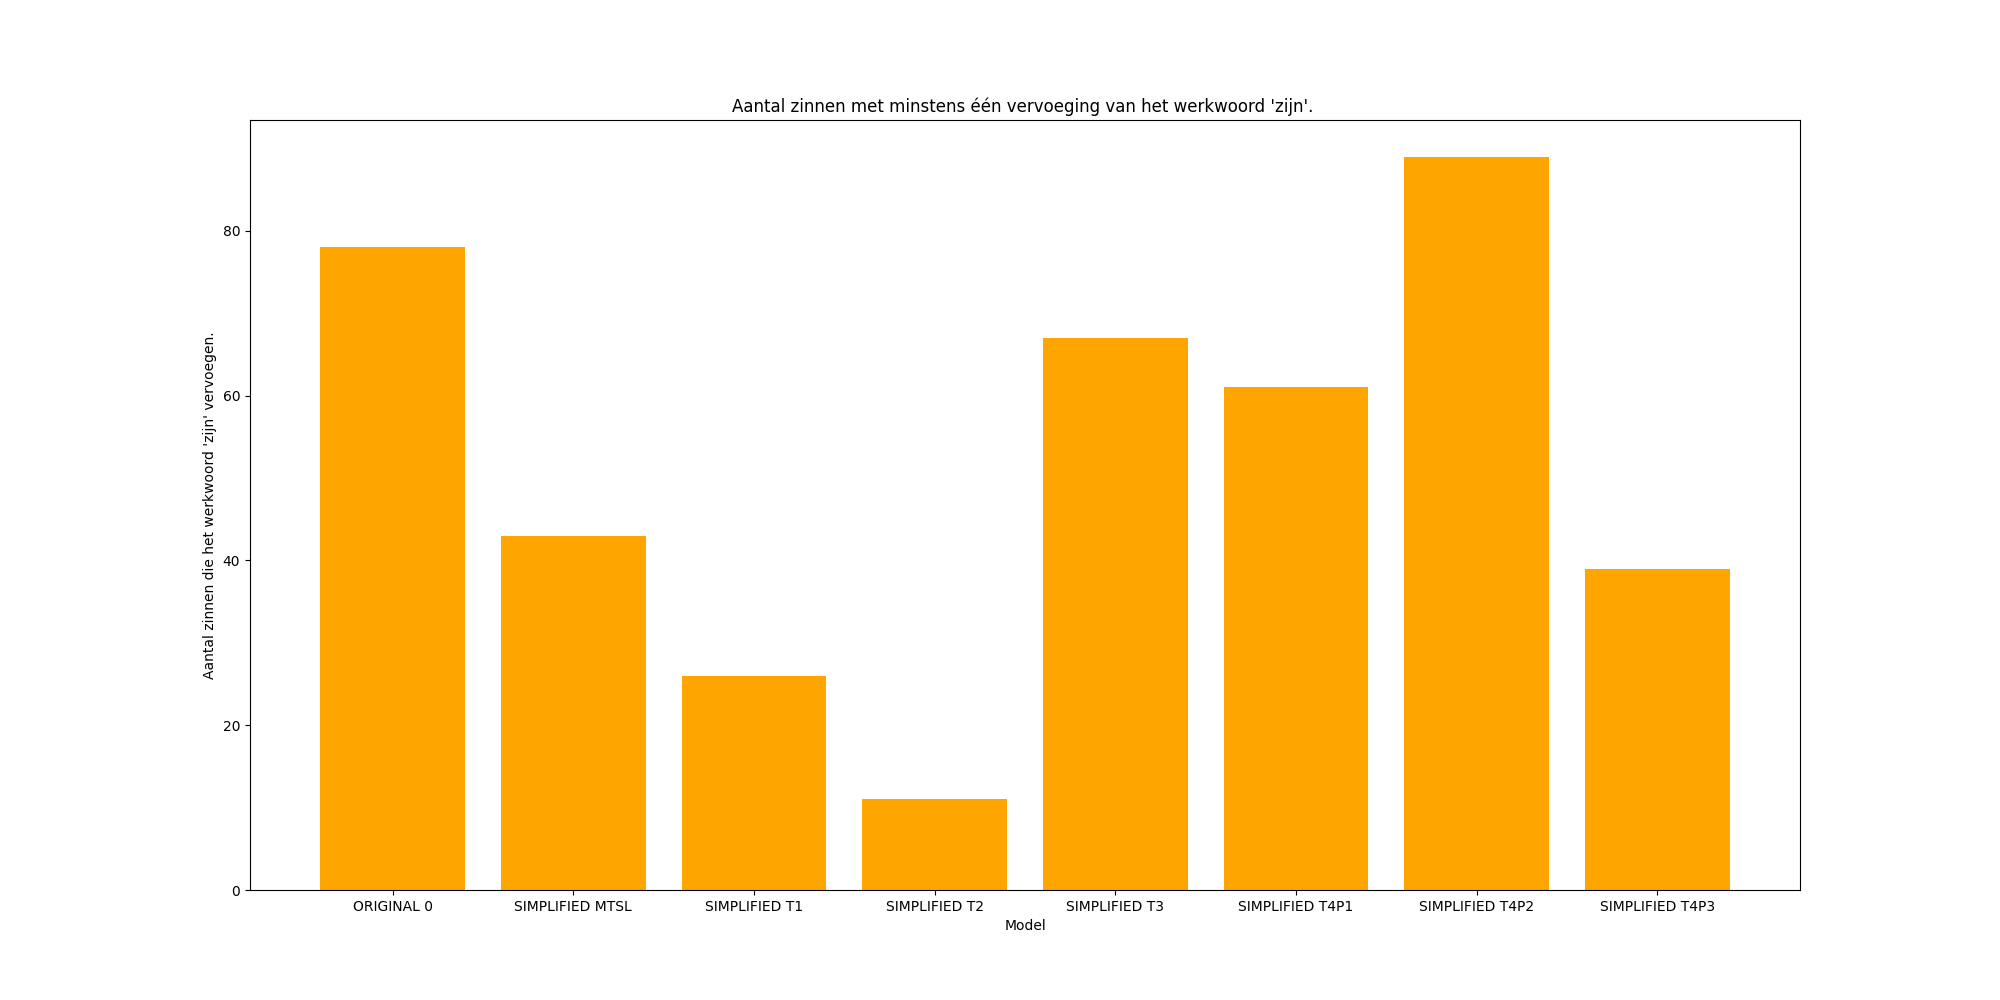
\includegraphics[width=\linewidth]{img/boxplot-tobe-a1.png}
	\caption{Gemiddeld aantal vervoegingen van het werkwoord 'zijn' per zin gegroepeerd op model voor A1.}
	\label{img:histplot-tobe-a1}
\end{figure}

\begin{figure}
	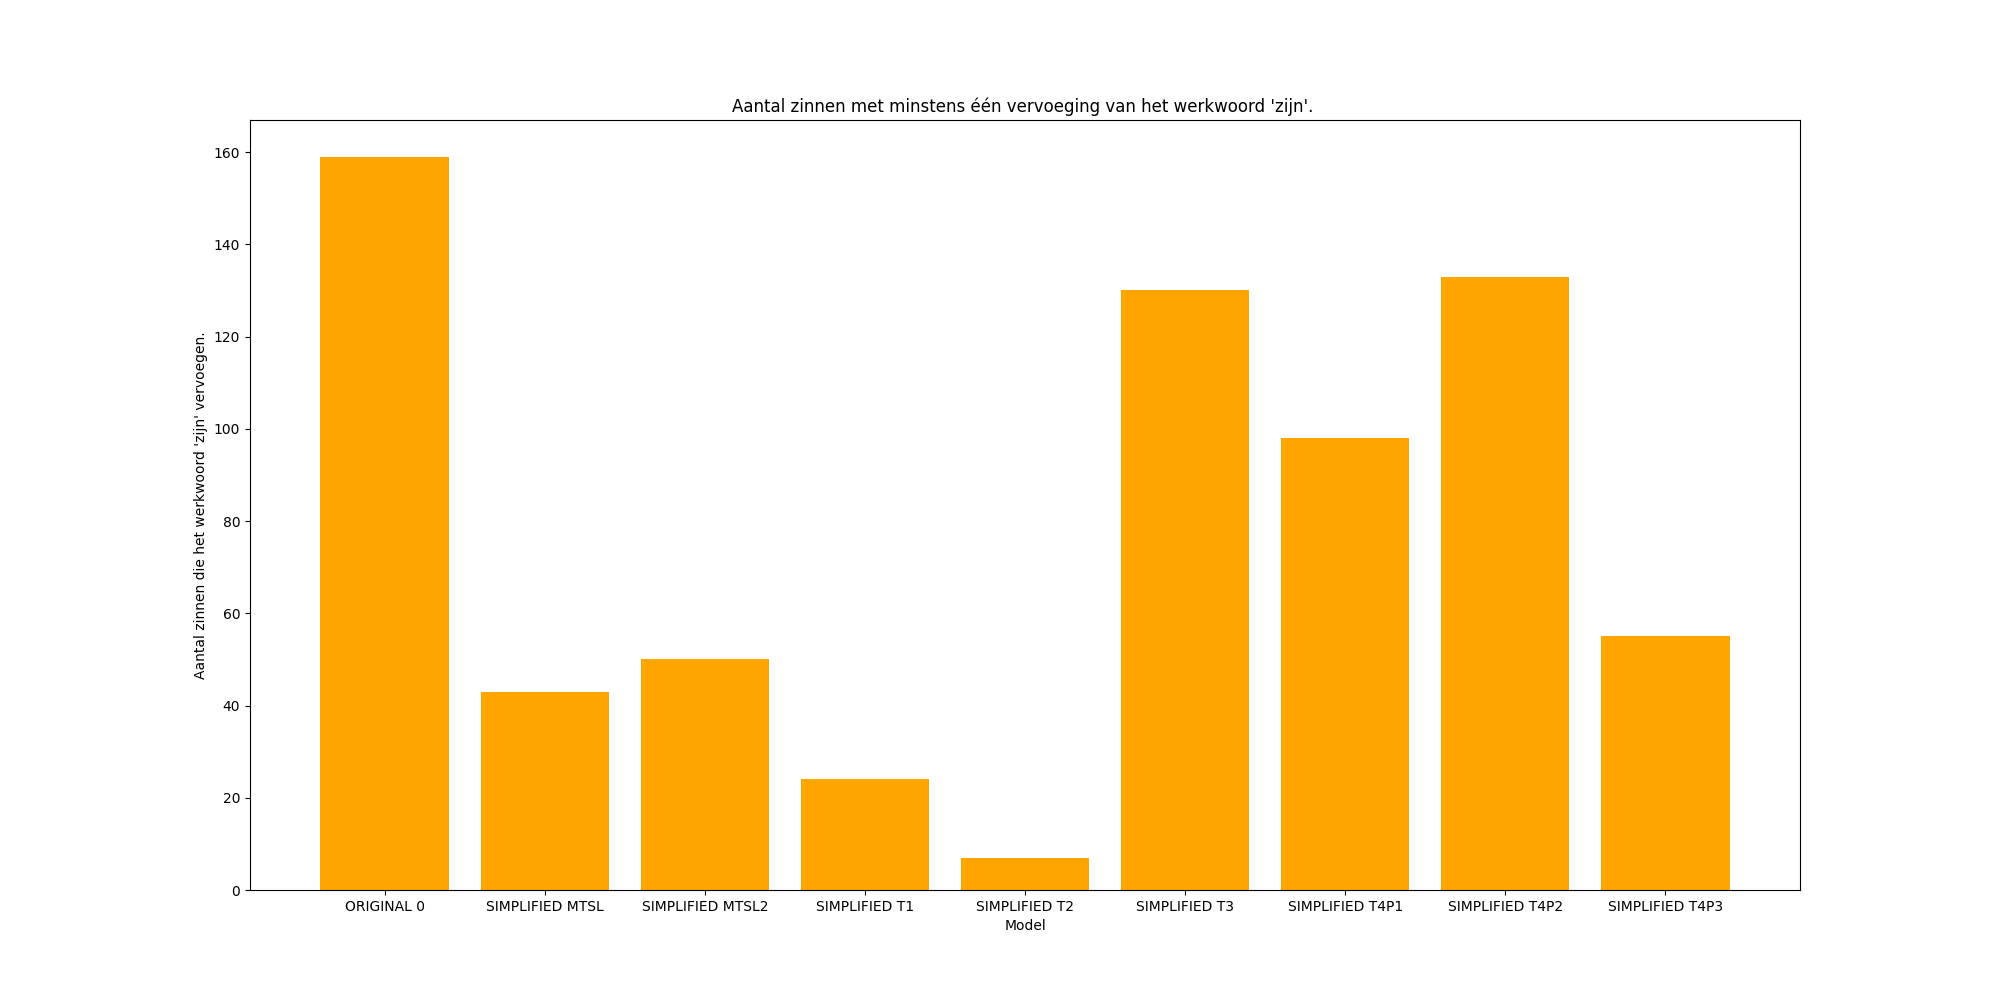
\includegraphics[width=\linewidth]{img/boxplot-tobe-a2.png}
	\caption{Gemiddeld aantal vervoegingen van het werkwoord 'zijn' per zin gegroepeerd op model voor A2.}
	\label{img:histplot-tobe-a2}
\end{figure}